\documentclass[12pt,english,dvipsnames,aspectratio=169,handout]{beamer}\usepackage[]{graphicx}\usepackage[]{xcolor}
% maxwidth is the original width if it is less than linewidth
% otherwise use linewidth (to make sure the graphics do not exceed the margin)
\makeatletter
\def\maxwidth{ %
  \ifdim\Gin@nat@width>\linewidth
    \linewidth
  \else
    \Gin@nat@width
  \fi
}
\makeatother

\definecolor{fgcolor}{rgb}{0.345, 0.345, 0.345}
\newcommand{\hlnum}[1]{\textcolor[rgb]{0.686,0.059,0.569}{#1}}%
\newcommand{\hlstr}[1]{\textcolor[rgb]{0.192,0.494,0.8}{#1}}%
\newcommand{\hlcom}[1]{\textcolor[rgb]{0.678,0.584,0.686}{\textit{#1}}}%
\newcommand{\hlopt}[1]{\textcolor[rgb]{0,0,0}{#1}}%
\newcommand{\hlstd}[1]{\textcolor[rgb]{0.345,0.345,0.345}{#1}}%
\newcommand{\hlkwa}[1]{\textcolor[rgb]{0.161,0.373,0.58}{\textbf{#1}}}%
\newcommand{\hlkwb}[1]{\textcolor[rgb]{0.69,0.353,0.396}{#1}}%
\newcommand{\hlkwc}[1]{\textcolor[rgb]{0.333,0.667,0.333}{#1}}%
\newcommand{\hlkwd}[1]{\textcolor[rgb]{0.737,0.353,0.396}{\textbf{#1}}}%
\let\hlipl\hlkwb

\usepackage{framed}
\makeatletter
\newenvironment{kframe}{%
 \def\at@end@of@kframe{}%
 \ifinner\ifhmode%
  \def\at@end@of@kframe{\end{minipage}}%
  \begin{minipage}{\columnwidth}%
 \fi\fi%
 \def\FrameCommand##1{\hskip\@totalleftmargin \hskip-\fboxsep
 \colorbox{shadecolor}{##1}\hskip-\fboxsep
     % There is no \\@totalrightmargin, so:
     \hskip-\linewidth \hskip-\@totalleftmargin \hskip\columnwidth}%
 \MakeFramed {\advance\hsize-\width
   \@totalleftmargin\z@ \linewidth\hsize
   \@setminipage}}%
 {\par\unskip\endMakeFramed%
 \at@end@of@kframe}
\makeatother

\definecolor{shadecolor}{rgb}{.97, .97, .97}
\definecolor{messagecolor}{rgb}{0, 0, 0}
\definecolor{warningcolor}{rgb}{1, 0, 1}
\definecolor{errorcolor}{rgb}{1, 0, 0}
\newenvironment{knitrout}{}{} % an empty environment to be redefined in TeX

\usepackage{alltt}
\usepackage{fontspec}
\setsansfont[Mapping=tex-text]{Fira Sans}
\setcounter{secnumdepth}{4}
\setcounter{tocdepth}{4}
\usepackage[normalem]{ulem}
\usepackage[T1]{fontenc}
\usepackage{dcolumn}
\usepackage{booktabs}
\usepackage{bm}
\usepackage{setspace}
\makeatletter
\usetheme{metropolis}
\setbeamertemplate{frame footer}{Bosancianu | Schaub | Hertie School}
\setbeamerfont{page number in head/foot}{size=\tiny}
\setbeamercolor{footline}{fg=gray}
\usepackage{xcolor}
\setbeamercovered{transparent}
\usepackage{tikz, tikz-cd}
\usetikzlibrary{arrows, positioning,fit,shapes.misc}
\usepackage[labelformat=empty]{caption}
% For table captions in Beamer
\usepackage[sectionbib]{apacite}
\renewcommand{\bibliographytypesize}{\footnotesize}
\makeatletter
\let\st@rtbibsection\@bibnewpage
\let\st@rtbibchapter\@bibnewpage
\makeatother
\usepackage{amsmath, mathtools}
\usepackage{xunicode}
\usepackage{hyperref, subcaption}
\graphicspath{{./figures/}} 
% Defines a checkmark
\def\checkmark{\tikz\fill[scale=0.4,color=orange](0,.35) -- (.25,0) -- (1,.7) -- (.25,.15) -- cycle;}
% Code for circles in Table cells
\newcounter{nodemarkers}
\newcommand\circletext[1]{%
    \tikz[overlay,remember picture] 
        \node (marker-\arabic{nodemarkers}-a) at (0,1.5ex) {};%
    #1%
    \tikz[overlay,remember picture]
        \node (marker-\arabic{nodemarkers}-b) at (0,0){};%
    \tikz[overlay,remember picture,inner sep=2pt]
        \node[draw,ellipse,fit=(marker-\arabic{nodemarkers}-a.center) (marker-\arabic{nodemarkers}-b.center)] {};%
    \stepcounter{nodemarkers}%
}
% wide itemize and enumerate
\newenvironment{wideitemize}{\itemize\addtolength{\itemsep}{.3em}}{\enditemize}
\newenvironment{wideenumerate}{\enumerate\addtolength{\itemsep}{.3em}}{\endenumerate}
% boxes
\def\boxitorange#1{%
  \smash{\color{orange}\fboxrule=1pt\relax\fboxsep=2pt\relax%
  \llap{\rlap{\fbox{\vphantom{0}\makebox[#1]{}}}~}}\ignorespaces
}
\def\boxitblue#1{%
  \smash{\color{blue}\fboxrule=1pt\relax\fboxsep=2pt\relax%
  \llap{\rlap{\fbox{\vphantom{0}\makebox[#1]{}}}~}}\ignorespaces
}
\setbeamertemplate{itemize items}{\checkmark}
\usepackage{multirow}
\hypersetup{pdfauthor={Bosancianu and Schaub},
	pdftitle={Statistical Modeling and Causal Inference with R},
	pdfsubject={Week 12: Field experiments},
	pdfkeywords={Berlin, Hertie, 2020, week 12, Field experiments}}
\title{\textsc{Statistical Modeling and Causal Inference with R}}
\subtitle{Week 12: Field experiments}
\date{November 30, 2020}
\author{Manuel Bosancianu \hfill Max Schaub}
\institute{Hertie School of Governance}
\IfFileExists{upquote.sty}{\usepackage{upquote}}{}
\begin{document}
\maketitle

\begin{frame}
	\frametitle{Today's focus}
	\begin{itemize}
		\item Intro
		\item DIY field experiments
		\item Challenges in field experiments
		\item Innovations in RCT design and implementation
	\end{itemize}
\end{frame}

\section{DIY field experiments}

\begin{frame}
	\frametitle{Perks of (DIY) field experiments}
	\begin{itemize}
		\item Evidence of causal effects on real-world behaviors
		\item Advance theory, e.g.\ importance of social norms
		\item Inform social policy (cp.\ Baldassarri and Abascal \citeyear{baldassarri_field_2017})
		\item Fun to plan and implement!
	\end{itemize}
\vspace{3cm}
\end{frame}


\begin{frame}
	\frametitle{DIY field experiments}
	\begin{enumerate}
	  \item Nudging interventions and GOTV
		\item Manipulation-of-context experiments 
		\item Lost letters
		\item Correspondence tests/audit studies
		\item Actor/conferderate-driven design
		\item Small-incentive design
		\item Lab-in-the-field experiments
	\end{enumerate}
\end{frame}


\begin{frame}
	\frametitle{1 Nudging interventions and GOTV}
	\footnotesize
\begin{itemize}
  \item Use small intervention (`nudge') to trigger behavioral change such as more environmentally friendly behavior \cite{nolan_normative_2008}, or higher turnout (get-out-the-vote or GOTV experiments) \cite{gerber_social_2008}
  \item Often uses i) social comparison, ii) `opt in' instead of `opt out', and/or iii) tests the effectiveness of different methods, e.g.\ in-person canvassing vs.\ phone calls (in GOTV experiments)
  \item Typically implemented within existing structures/procedures, e.g.\ existing business practices, planned election campaigns
  \item Cheap -- if you can convince someone to randomize treatments 
\end{itemize}
\vspace{3cm}
\end{frame}



\begin{frame}
	\frametitle{Example: Goldstein, Cialdini, and Griskevicius \citeyear{goldstein_room_2008}}
    \begin{figure}[ht]
        \begin{minipage}[b]{0.35\linewidth}
            \centering
            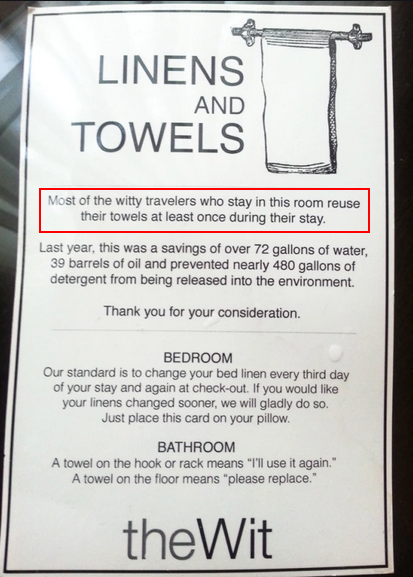
\includegraphics[width=\textwidth]{../04-figures/12/09-w12_nudge14}
        \end{minipage}
        \hspace{0.5cm}
        \begin{minipage}[b]{0.4\linewidth}
            \centering
            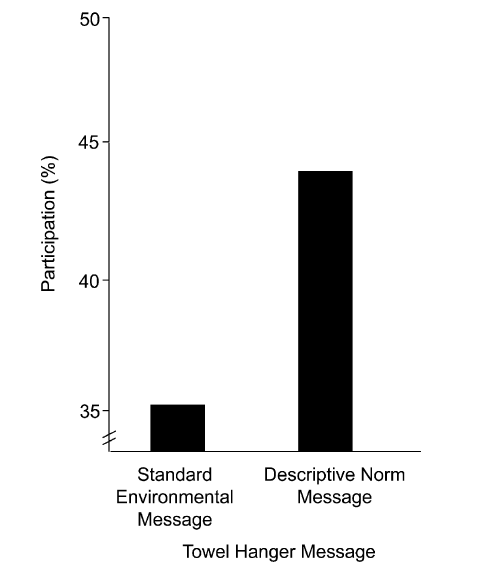
\includegraphics[width=\textwidth]{../04-figures/12/10-w12_nudge13}
        \end{minipage}
    \end{figure}
\end{frame}


\begin{frame}
	\frametitle{2 Manipulation-of-context experiments}
	\footnotesize
\begin{itemize}
  \item Manipulate context to elicit changes in behavior
  \item Most famously used to test `broken windows' theory, i.e.\ the idea that disorderly environments cause norm violations
  \item Fascinating, easy to implement -- but limited applicability (?)
\end{itemize}
\vspace{3cm}
\end{frame}


\begin{frame}
	\frametitle{Example: Keizer, Lindeberg, and Steg \citeyear{keizer_spreading_2008}}
    \begin{figure}[ht]
        \begin{minipage}[b]{0.45\linewidth}
            \centering
            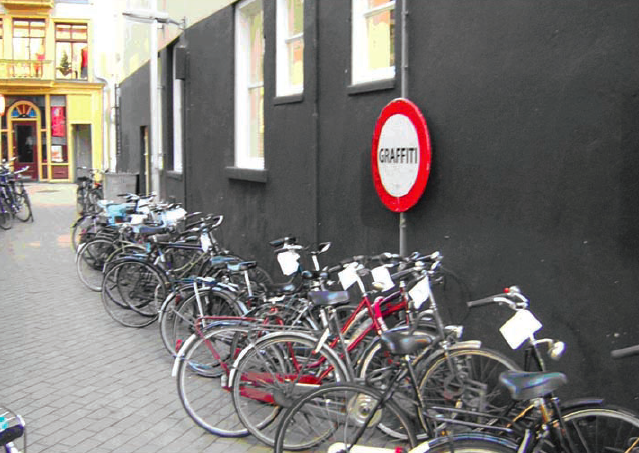
\includegraphics[width=\textwidth]{../04-figures/12/11-w12_disorder1}
        \end{minipage}
        \hspace{0.5cm}
        \begin{minipage}[b]{0.45\linewidth}
            \centering
            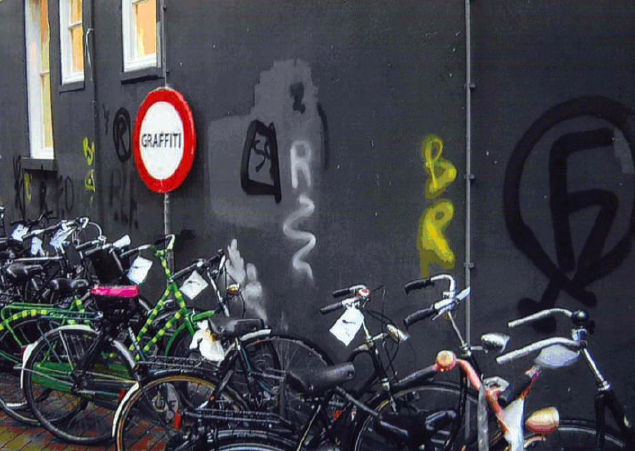
\includegraphics[width=\textwidth]{../04-figures/12/12-w12_disorder12}
        \end{minipage}
    \end{figure}
\end{frame}


\begin{frame}
	\frametitle{3 Lost letters}
	\footnotesize
\begin{itemize}
  \item Letters with an address and stamp are distributed in neighborhoods; outcome is return rate \cite{milgram_lostletter_1965}
  \item Either used to test for the effect of context, e.g.\ ethnically diverse \cite{koopmans_cooperation_2014}, high vs.\ low market integration (but: not randomized!), or to probe for discrimination e.g.\ against foreigners, politicians (easy to randomize)
  \item Fairly cheap to implement, needs careful planning (distance to post boxes, weather, etc.)
\end{itemize}
\vspace{3cm}
\end{frame}


\begin{frame}
	\frametitle{Example: Baldassarri \citeyear{baldassarri_market_2020}}
    \begin{figure}[ht]
        \begin{minipage}[b]{0.45\linewidth}
            \centering
            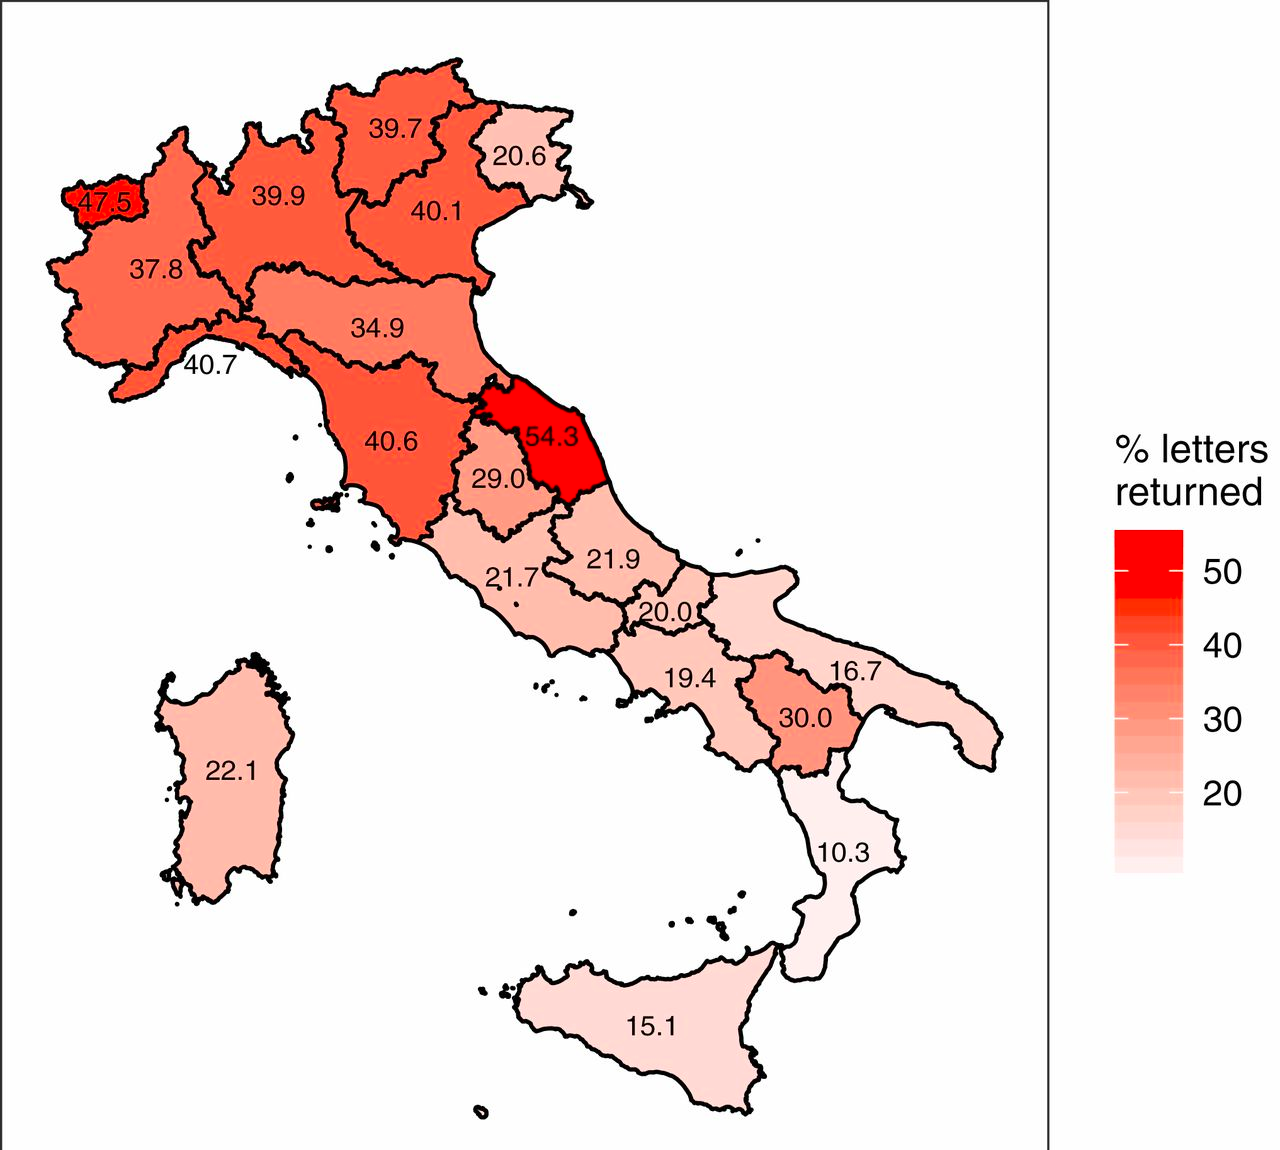
\includegraphics[width=\textwidth]{../04-figures/12/13-w12_lostletter2}
        \end{minipage}
        \hspace{0.5cm}
        \begin{minipage}[b]{0.45\linewidth}
            \centering
            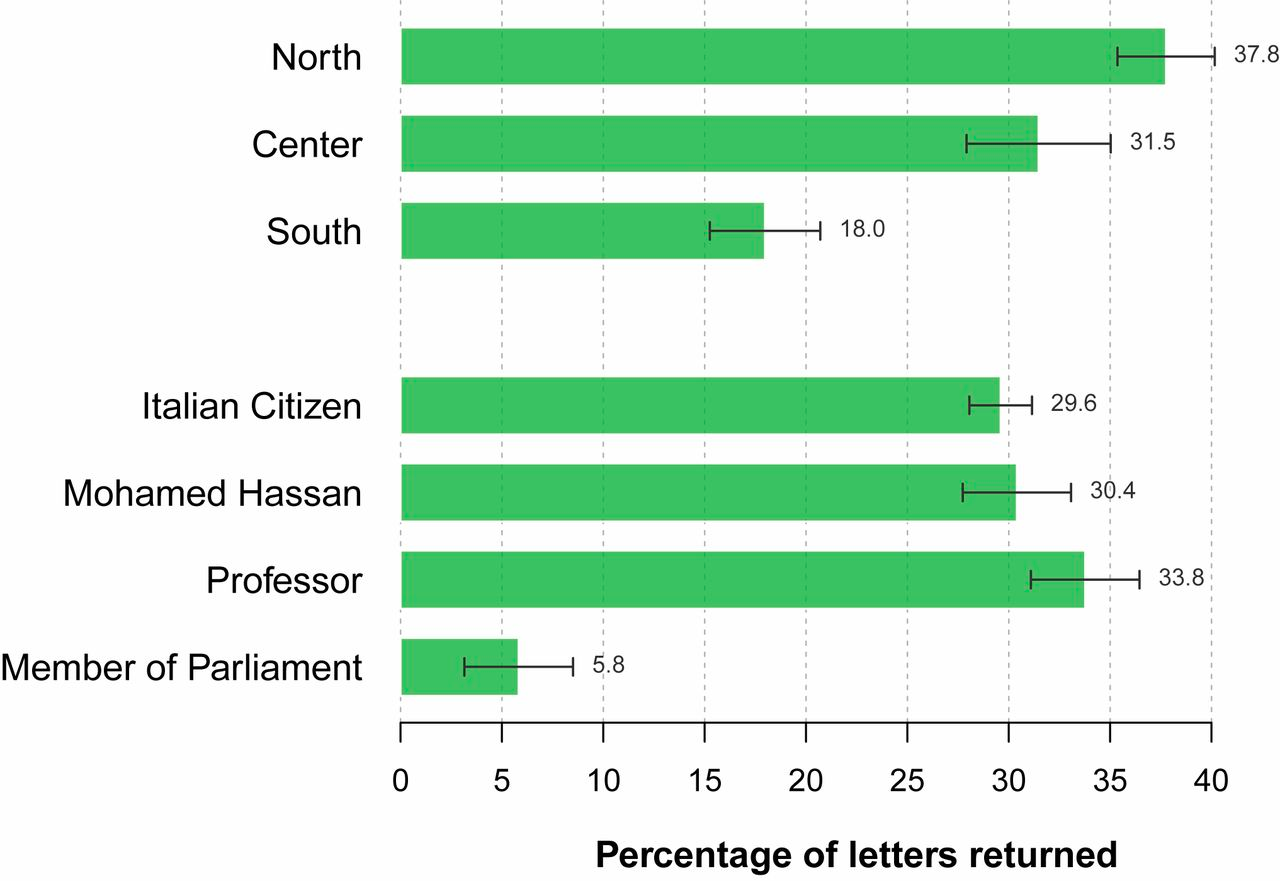
\includegraphics[width=\textwidth]{../04-figures/12/14-w12_lostletter1}
        \end{minipage}
    \end{figure}
\end{frame}



\begin{frame}
	\frametitle{4 Correspondence tests/audit studies}
	\footnotesize
\begin{itemize}
  \item Manipulate correspondence with potential employers \cite{bertrand_are_2004}, landlords \cite{bartos_attention_2016}, state institutions \cite{hemker_multiple_2017}
  \item Classic method to test for discrimination in terms of ethnicity, sex, etc. 
  \item Labor intense but fairly cheap, especially when using electronic correspondence
\end{itemize}
\vspace{3cm}
\end{frame}


\begin{frame}
	\frametitle{Example: Koopmans, Veit, and Yemane \citeyear{koopmans_taste_2019} }
    \begin{figure}[t]
        \begin{minipage}[b]{0.5\linewidth}
            \centering
            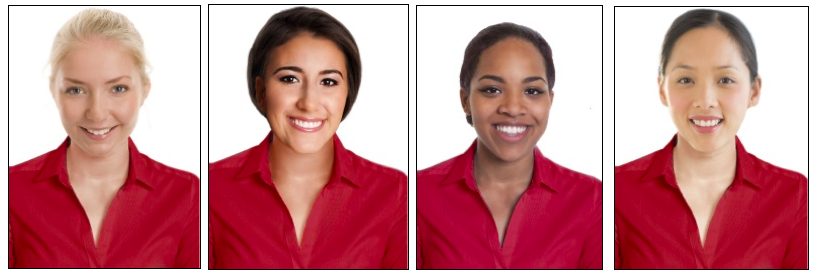
\includegraphics[width=0.9\textwidth]{../04-figures/12/15-w12_correpondence2}
        \end{minipage}
        \hspace{0.5cm}
        \begin{minipage}[b]{0.5\linewidth}
            \centering
            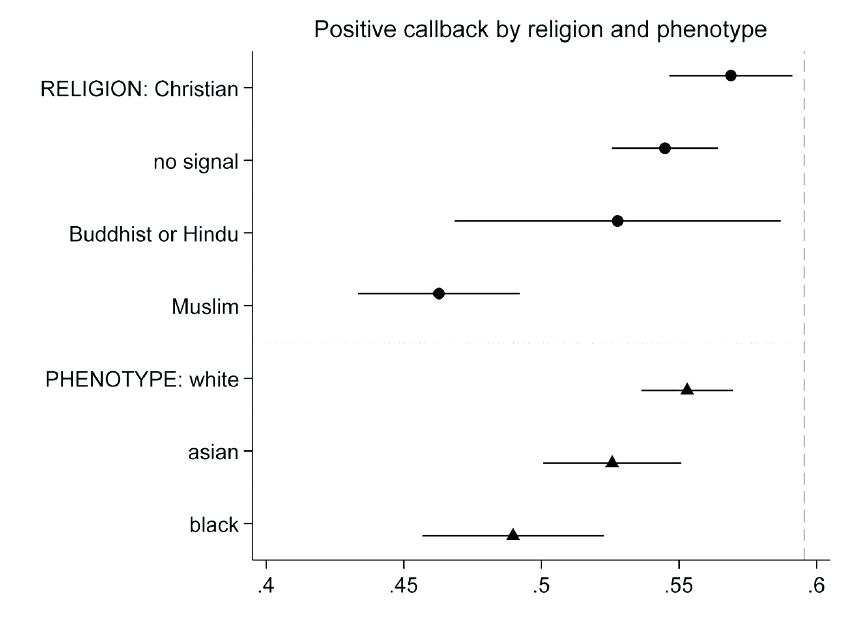
\includegraphics[width=0.9\textwidth]{../04-figures/12/16-w12_correpondence1}
        \end{minipage}
    \end{figure}
\end{frame}



\begin{frame}
	\frametitle{5 Actor/confederate-driven design}
	\footnotesize
\begin{itemize}
  \item Have confederates (trained actors or layperson), record reaction of public
  \item Used to study social norms \cite{cohen_field_1997, winter_social_2018}, anti-immigrant sentiments \cite{enos_causal_2014}, etc.
  \item Effective method if done well, limited applications (?)
\end{itemize}
\vspace{3cm}
\end{frame}


\begin{frame}
	\frametitle{Example: Winter and Zhang \citeyear{winter_social_2018}}
    \begin{figure}[ht]
        \begin{minipage}[b]{0.6\linewidth}
            \centering
            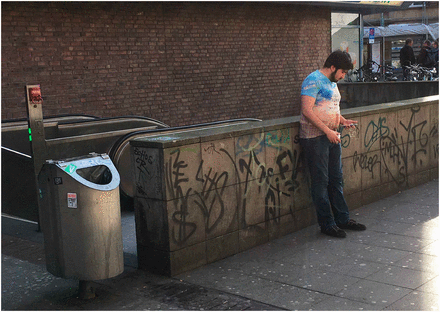
\includegraphics[width=\textwidth]{../04-figures/12/17-w12_actor}
        \end{minipage}
        \hspace{0.5cm}
        \begin{minipage}[b]{0.25\linewidth}
            \centering
            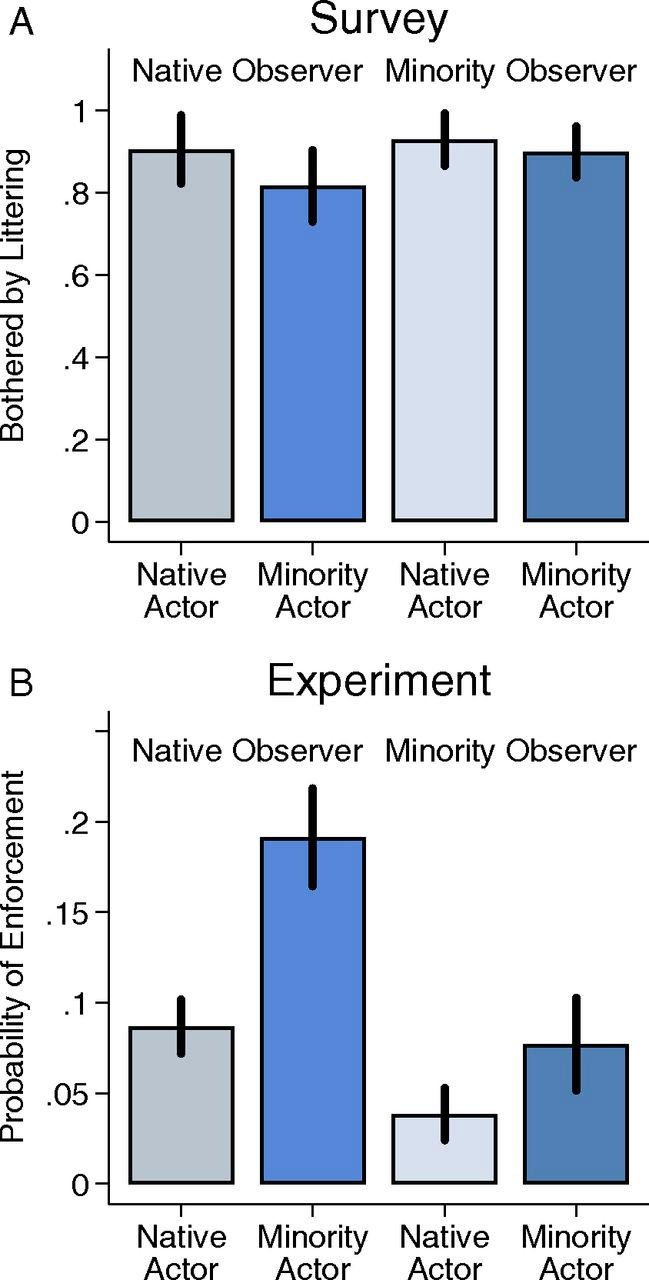
\includegraphics[width=\textwidth]{../04-figures/12/18-w12_actor_results}
        \end{minipage}
    \end{figure}
\end{frame}



\begin{frame}
	\frametitle{6 Small-incentive design}
	\footnotesize
\begin{itemize}
  \item Small monetary incentive to encourage change in behavior in large range of domains, from compliance with rules for picking up kids from daycare \cite{gneezy_fine_2000} to migration \cite{bryan_underinvestment_2014}
  \item Incentive can we positive (reward) or negative (fine) 
  \item Very flexible, but not so cheap in the case of rewards (small incentives can add up!) 
\end{itemize}
\vspace{3cm}
\end{frame}


\begin{frame}
	\frametitle{Example: Batista and Narciso \citeyear{batista_migrant_2013}}
    \begin{figure}[ht]
        \begin{minipage}[b]{0.3\linewidth}
            \centering
            
\includegraphics[width=\textwidth]{../04-figures/12/19-w12_callcredit2}
        \end{minipage}
        \hspace{0.5cm}
        \begin{minipage}[b]{0.6\linewidth}
            \centering
            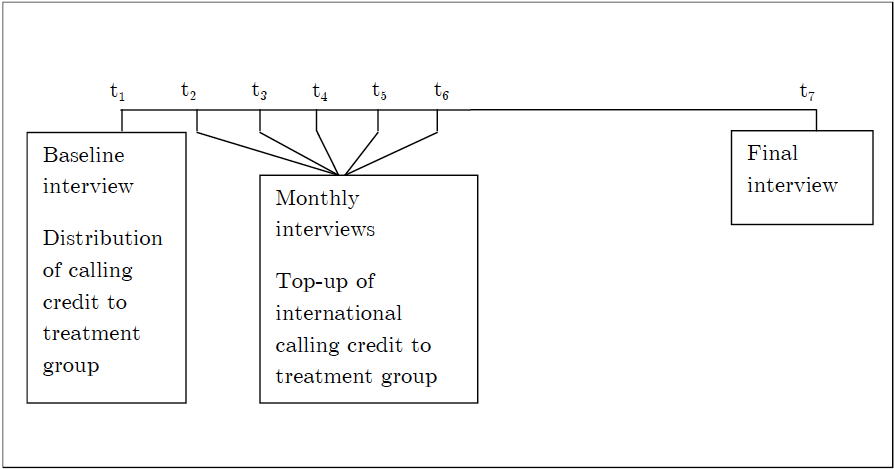
\includegraphics[width=\textwidth]{../04-figures/12/20-w12_callcredit}
        \end{minipage}
    \end{figure}
\end{frame}



\begin{frame}
	\frametitle{7 Lab-in-the-field experiments}
	\footnotesize
\begin{itemize}
\item Use of behavioral games (dictator game, trust game, PGG) typically employed in econ labs in field settings
  \item Used to measure cooperative \cite{baldassarri_centralized_2011}, spiteful \cite{prediger_resource_2014},  intergroup \cite{abascal_us_2015}, and other types of behavior in abstract (and putatively generalizable) way
  \item Blend of controlled lab environment with field setting (i.e.\ `bringing the lab to the field') 
  \item Somewhat specialized type of research; needs careful preparation and buy in; protocols for standard games widely available; but not for free (behavioral games usually entail incentives).
\end{itemize}
\vspace{3cm}
\end{frame}


\begin{frame}
	\frametitle{Example: Habyarimana et al.\ \citeyear{habyarimana_why_2007}}
    \begin{figure}[ht]
        \begin{minipage}[b]{0.5\linewidth}
            \centering
            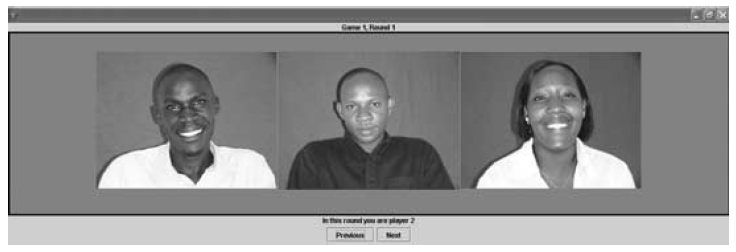
\includegraphics[width=\textwidth]{../04-figures/12/21-w12_coethnicity}
        \end{minipage}
        \hspace{0.5cm}
        \begin{minipage}[b]{0.5\linewidth}
            \centering
            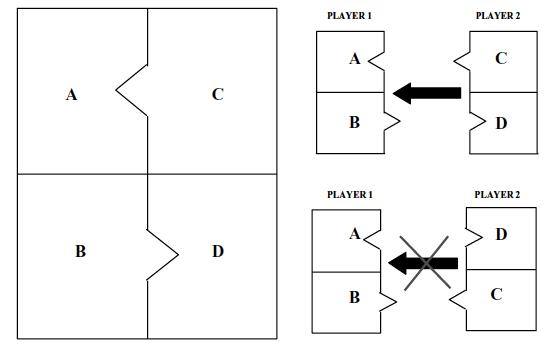
\includegraphics[width=\textwidth]{../04-figures/12/22-w12_puzzle}
        \end{minipage}
    \end{figure}
\end{frame}


\section{Challenges to RCT-based inference}

\begin{frame}
  \frametitle{RCT-based inference: vulnerabilities}
  Evidence of impressive creativity and flexibility in applying field experiments to substantive questions.\bigskip
  \pause
  
  Some hesitation about the potential of turning into a glorified form of policy analysis \cite{bates_banerjees_2006}.\bigskip
  \pause
  
  Concerns about inference \cite{humphreys_aggregation_2020}:
  
  \begin{itemize}
    \item external validity: Metaketa initiative;
    \item external validity: ``patient-preference''/selective trials;
    \item aggregation challenge: structural models
  \end{itemize}
  
\end{frame}


\subsection{External validity I}

\begin{frame}
  \frametitle{M\"{u}ller-Lyer illusion}
Which one is longer?\bigskip

\begin{figure}
\centering
\begin{subfigure}[c]{.4\textwidth}
\begin{tikzpicture}[scale=0.8]
\node[draw=none,inner sep=0pt,minimum size=1pt] (D) at (1,0) {};
\node[draw=none,inner sep=0pt,minimum size=1pt] (E) at (5,0) {};
\draw[-,very thick,color=orange] (D)--(E);
\node[draw=none] (C5) at (2,0.75) {};
\node[draw=none] (C6) at (2,-0.75) {};
\draw[-,very thick,color=black] (C5)--(D);
\draw[-,very thick,color=black] (C6)--(D);
\node[draw=none] (C7) at (4,0.75) {};
\node[draw=none] (C8) at (4,-0.75) {};
\draw[-,very thick,color=black] (E)--(C7);
\draw[-,very thick,color=black] (E)--(C8);
\end{tikzpicture}
\end{subfigure}
\begin{subfigure}[c]{.4\textwidth}
\begin{tikzpicture}[scale=0.8]
\node[draw=none,inner sep=0pt,minimum size=1pt] (A) at (1,0) {};
\node[draw=none,inner sep=0pt,minimum size=1pt] (B) at (5,0) {};
\draw[-,very thick,color=orange] (A)--(B);
\node[draw=none] (C1) at (0,0.75) {};
\node[draw=none] (C2) at (0,-0.75) {};
\draw[-,very thick,color=black] (C1)--(A);
\draw[-,very thick,color=black] (C2)--(A);
\node[draw=none] (C3) at (6,0.75) {};
\node[draw=none] (C4) at (6,-0.75) {};
\draw[-,very thick,color=black] (B)--(C3);
\draw[-,very thick,color=black] (B)--(C4);
\end{tikzpicture}
\end{subfigure}
\end{figure}\bigskip

We've known about this illusion since 1889. However, since 1966 we also know that not all cultures experience this in the same way.
\end{frame}


\begin{frame}
  \frametitle{Cross-cultural variance}

\citeA{segall_influence_1966} find differences between cultures in how different people perceive these lines to be.

\begin{figure}
\centering
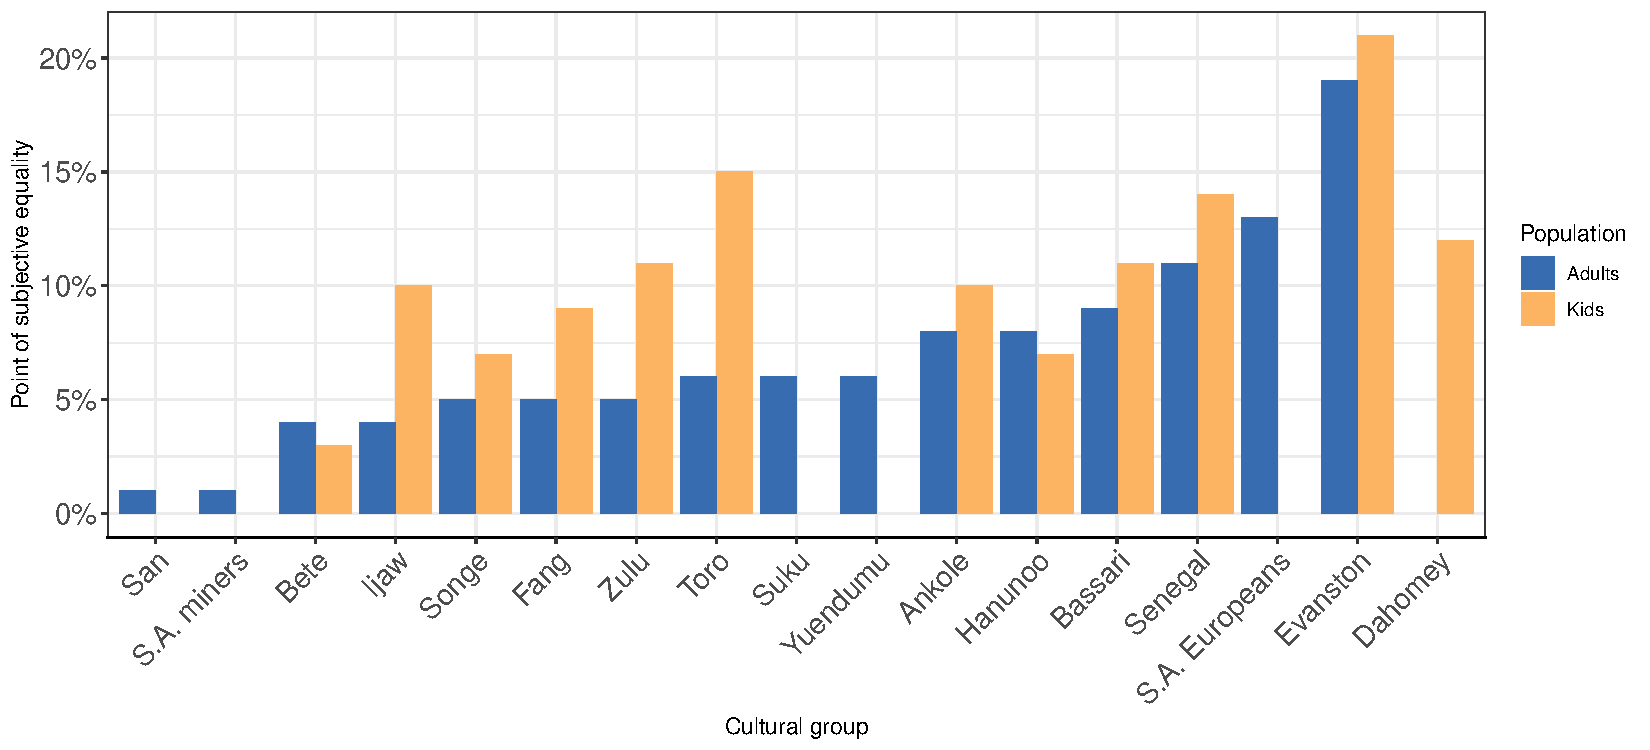
\includegraphics[scale=0.35]{../04-figures/12/01.pdf}
\caption*{Adapted from \citeA{mccauley_susceptibility_2006}}
\end{figure}
\end{frame}



\begin{frame}
  \frametitle{External validity concerns}
  Validity \cite{campbell_experimental_1966}:
  
  \begin{itemize}
    \item \textcolor{orange}{internal}: ability of design to capture actual magnitude of relationship in real life \pause
    \item \textcolor{orange}{external}: extent to which we can generalize measured effect to other populations, contexts, and ways of measuring phenomenon
  \end{itemize}\bigskip
  \pause
  
  Many choices in RCTs: treatment arms and delivery, study population, ways of measuring outcomes (attitudes, behavior, task-based).\bigskip
  \pause
  
  Professional incentives for innovation in study design (``plant the flag''), rather than replication.
\end{frame}


\begin{frame}
	\frametitle{Metaketa initiative}
	
	\begin{table}
		\scriptsize
		\begin{tabular}{p{6cm} p{4.5cm}}
			\toprule
			\textbf{Challenges} & \textbf{Features} \\
			\midrule
			Potential for confounding in observational research & RCTs \\
			Limited external validity of RCTs & Multiple studies across sites \\
			Heterogeneous, scattered findings & Meta-analysis for findings \\
			Diversity of interventions & ``Common arm'' intervention \\
			Noncomparable measurement & Harmonized measurement of inputs, outcomes, and controls \\
			Researcher incentives for innovation & ``Alternative arm'' intervention \\
			Private data & Open data and replication code \\
			Errors in data or code & Third-party data analysis \\
			Data fishing & Pre-analysis plans \\
			Publication bias & Publication of all registered analyses \\
			\bottomrule
		\end{tabular}
	\caption{Adapted from \citeA{dunning_metaketa_2019}}
	\end{table}
	
\end{frame}


\begin{frame}
	\frametitle{Metaketa I: information and accountability}
	
	\begin{table}
		\scriptsize
		\begin{tabular}{p {1.6cm} p{4cm} p{4.4cm}}
			\toprule
			\textbf{Site} & \textbf{Common arm} & \textbf{Alternative arm} \\
			\midrule
			Benin & Legislative performance & Civic lesson about legislative performance \\
			Brazil & Accounting irregularities & Municipal education outcomes \\
			Burkina Faso & Quality of municipal services & Invitation to municipal gov't meetings \\
			India & Criminal background of candidates (info. from enumerators) & Criminal background (info. from local brokers) \\
			Mexico & Unauthorized / misallocated spending & Misallocated spending (loudspeakers, or no benchmark ) \\
			Uganda 1 & Voter--candidate policy alignment (campaign videos) & Public provision of information \\
			Uganda 2& Budget irregularities (vias SMS) & Quality of service provision \\
			\bottomrule
		\end{tabular}
		\caption{Adapted from \citeA{dunning_metaketa_2019}}
	\end{table}
	
\end{frame}


\begin{frame}
	\frametitle{Results: information on turnout}
	
	\begin{figure}
		\centering
		\begin{subfigure}{0.47\linewidth}
			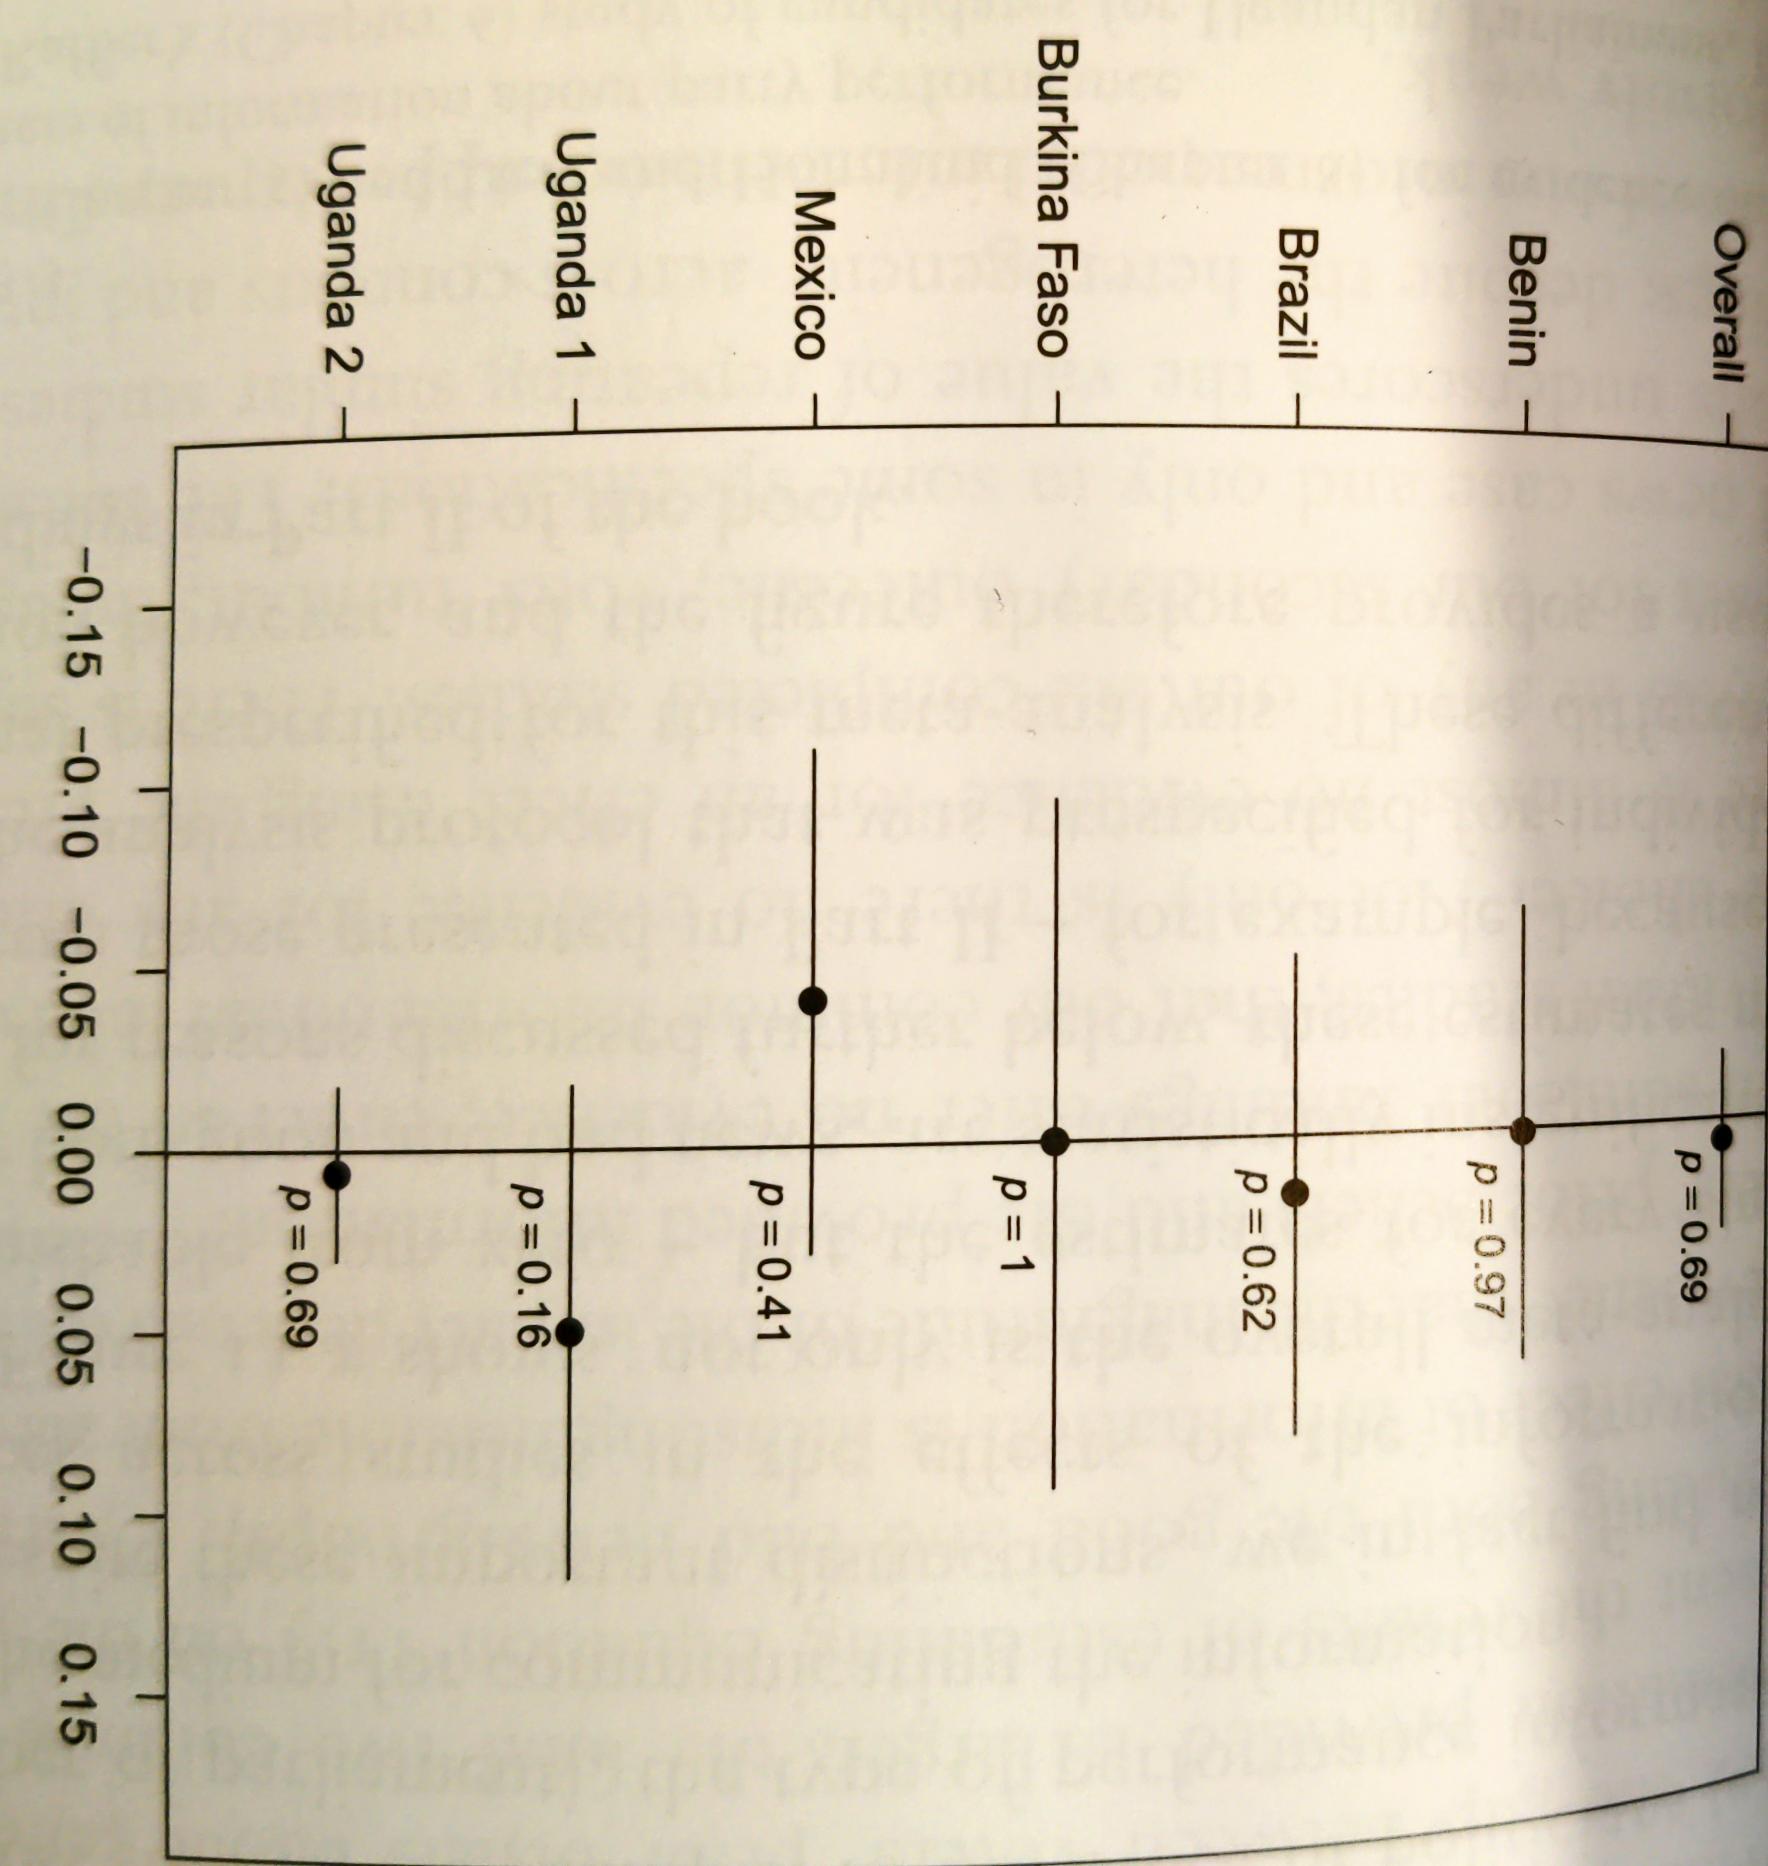
\includegraphics[scale=0.075,angle=90]{../04-figures/12/02-Good-news-choice.jpg}
			\caption{Good news}
		\end{subfigure}
	    \begin{subfigure}{0.47\linewidth}
	    	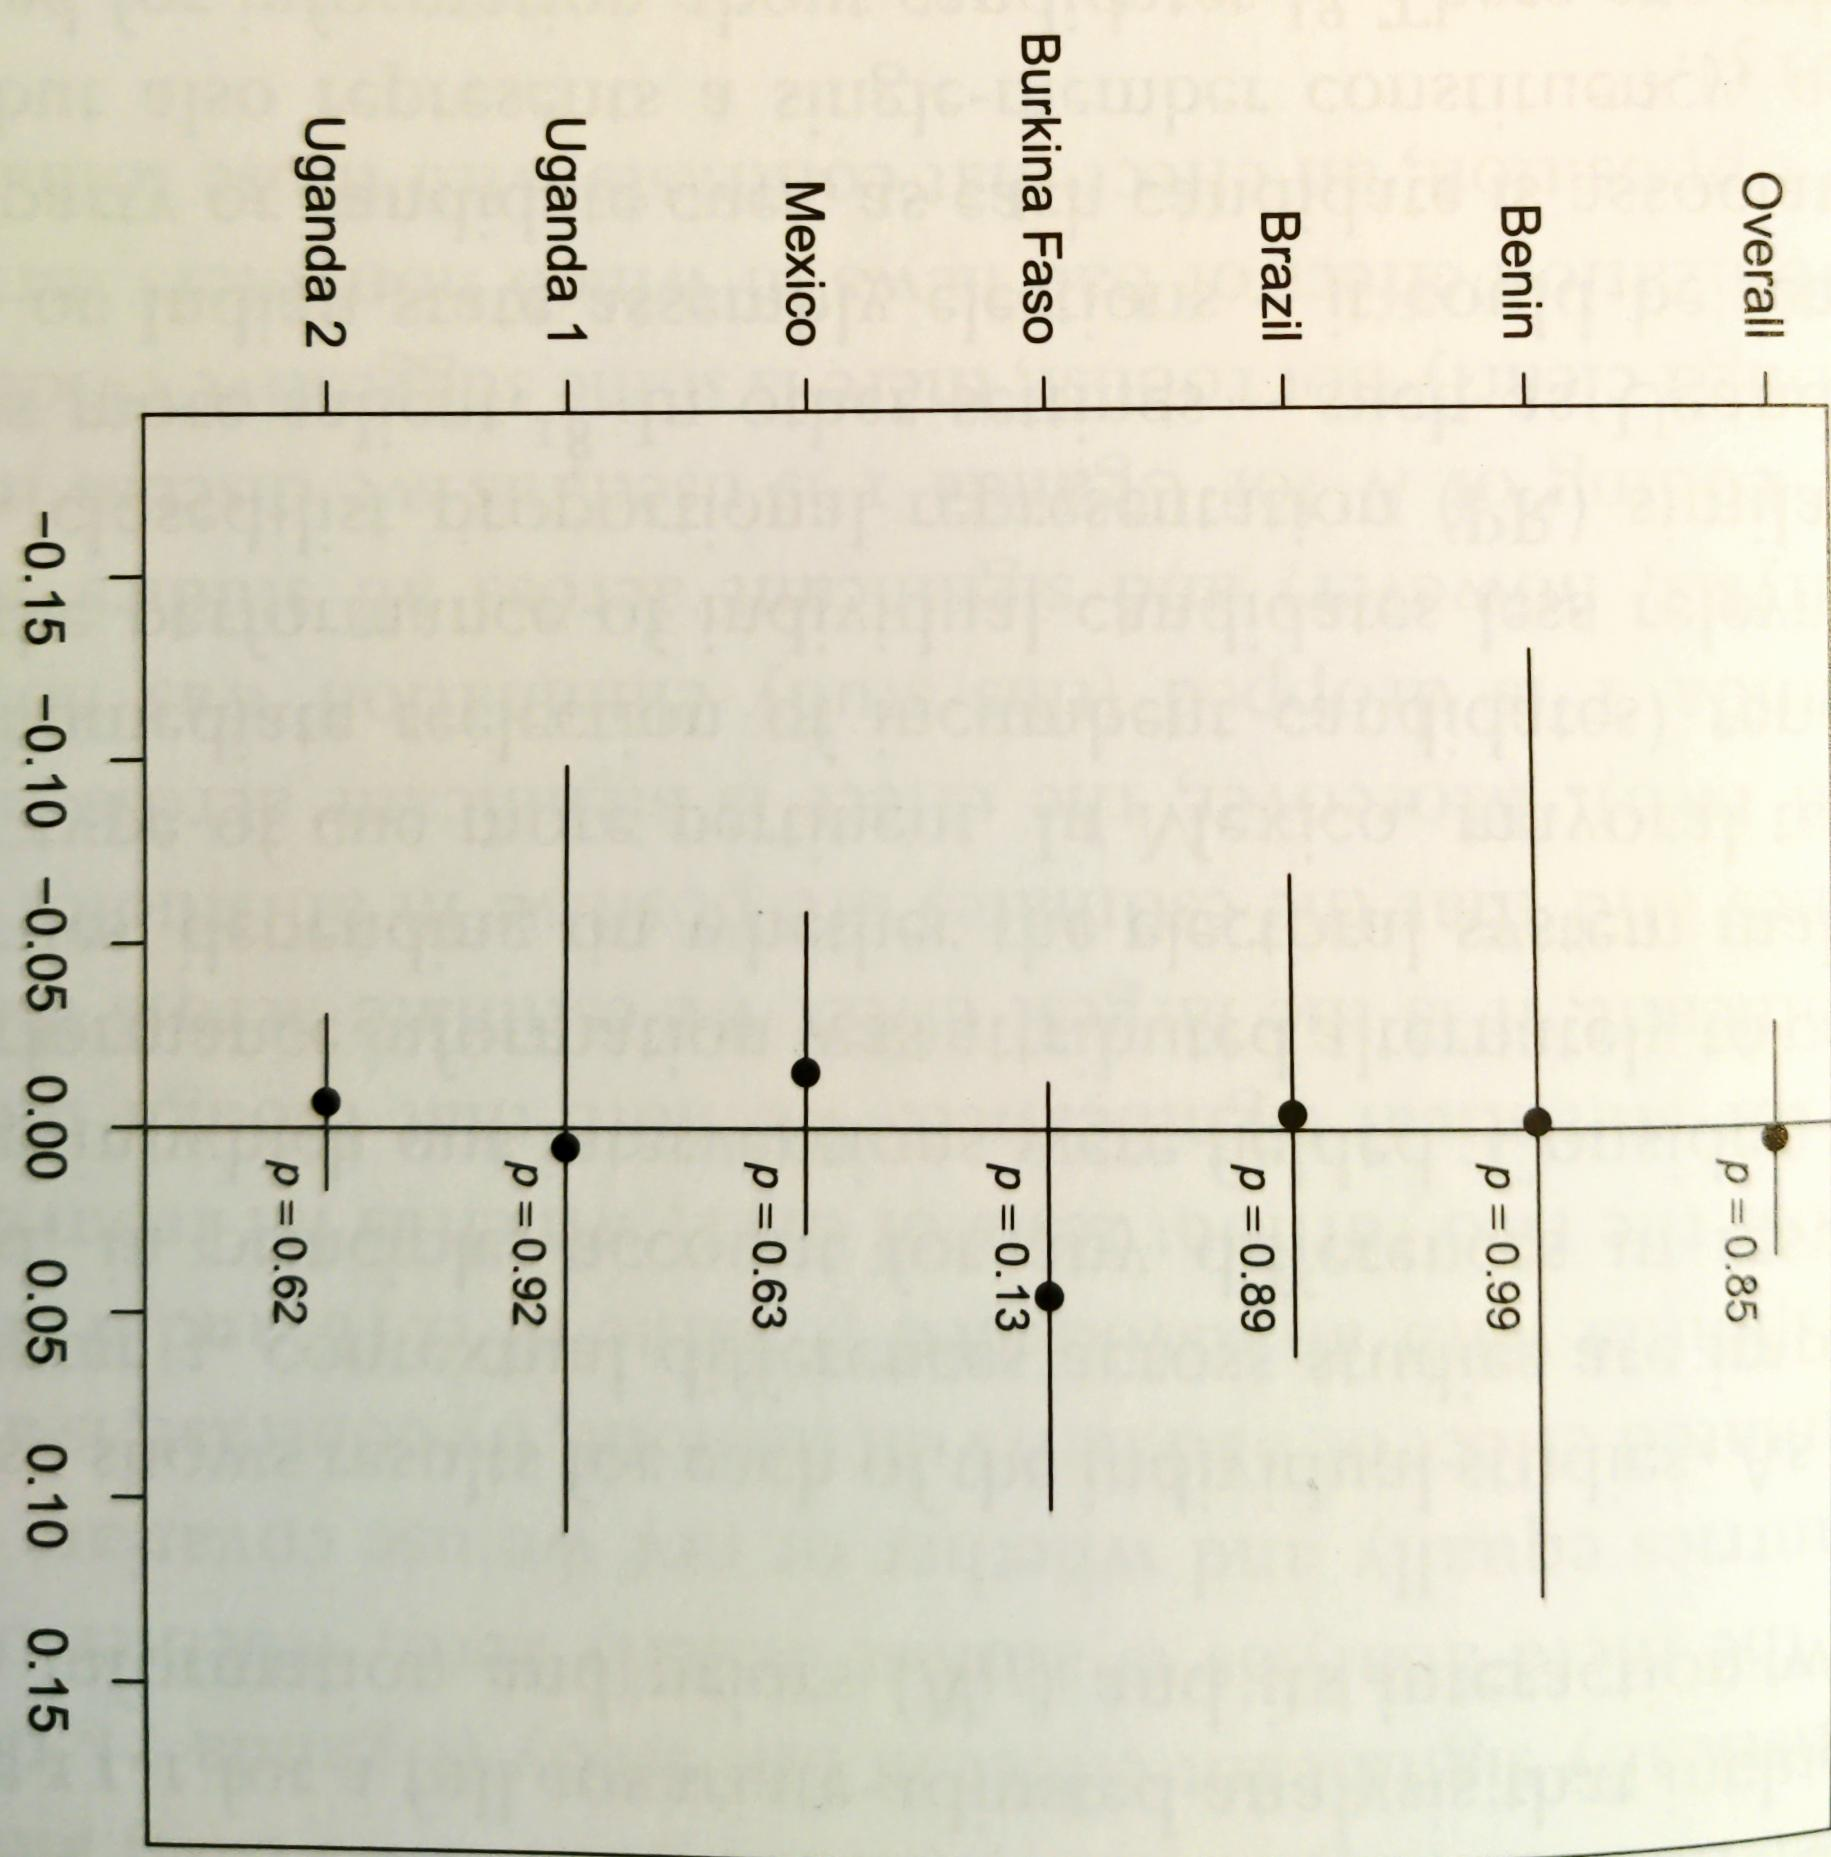
\includegraphics[scale=0.074,angle=90]{../04-figures/12/03-Bad-news-choice.jpg}
	    	\caption{Bad news}
	    \end{subfigure}
    \caption{Taken from \citeA{dunning_meta-analysis_2019}}
	\end{figure}
	
\end{frame}


\begin{frame}
	\frametitle{Results: information on vote choice}
	
	\begin{figure}
		\centering
		\begin{subfigure}{0.47\linewidth}
			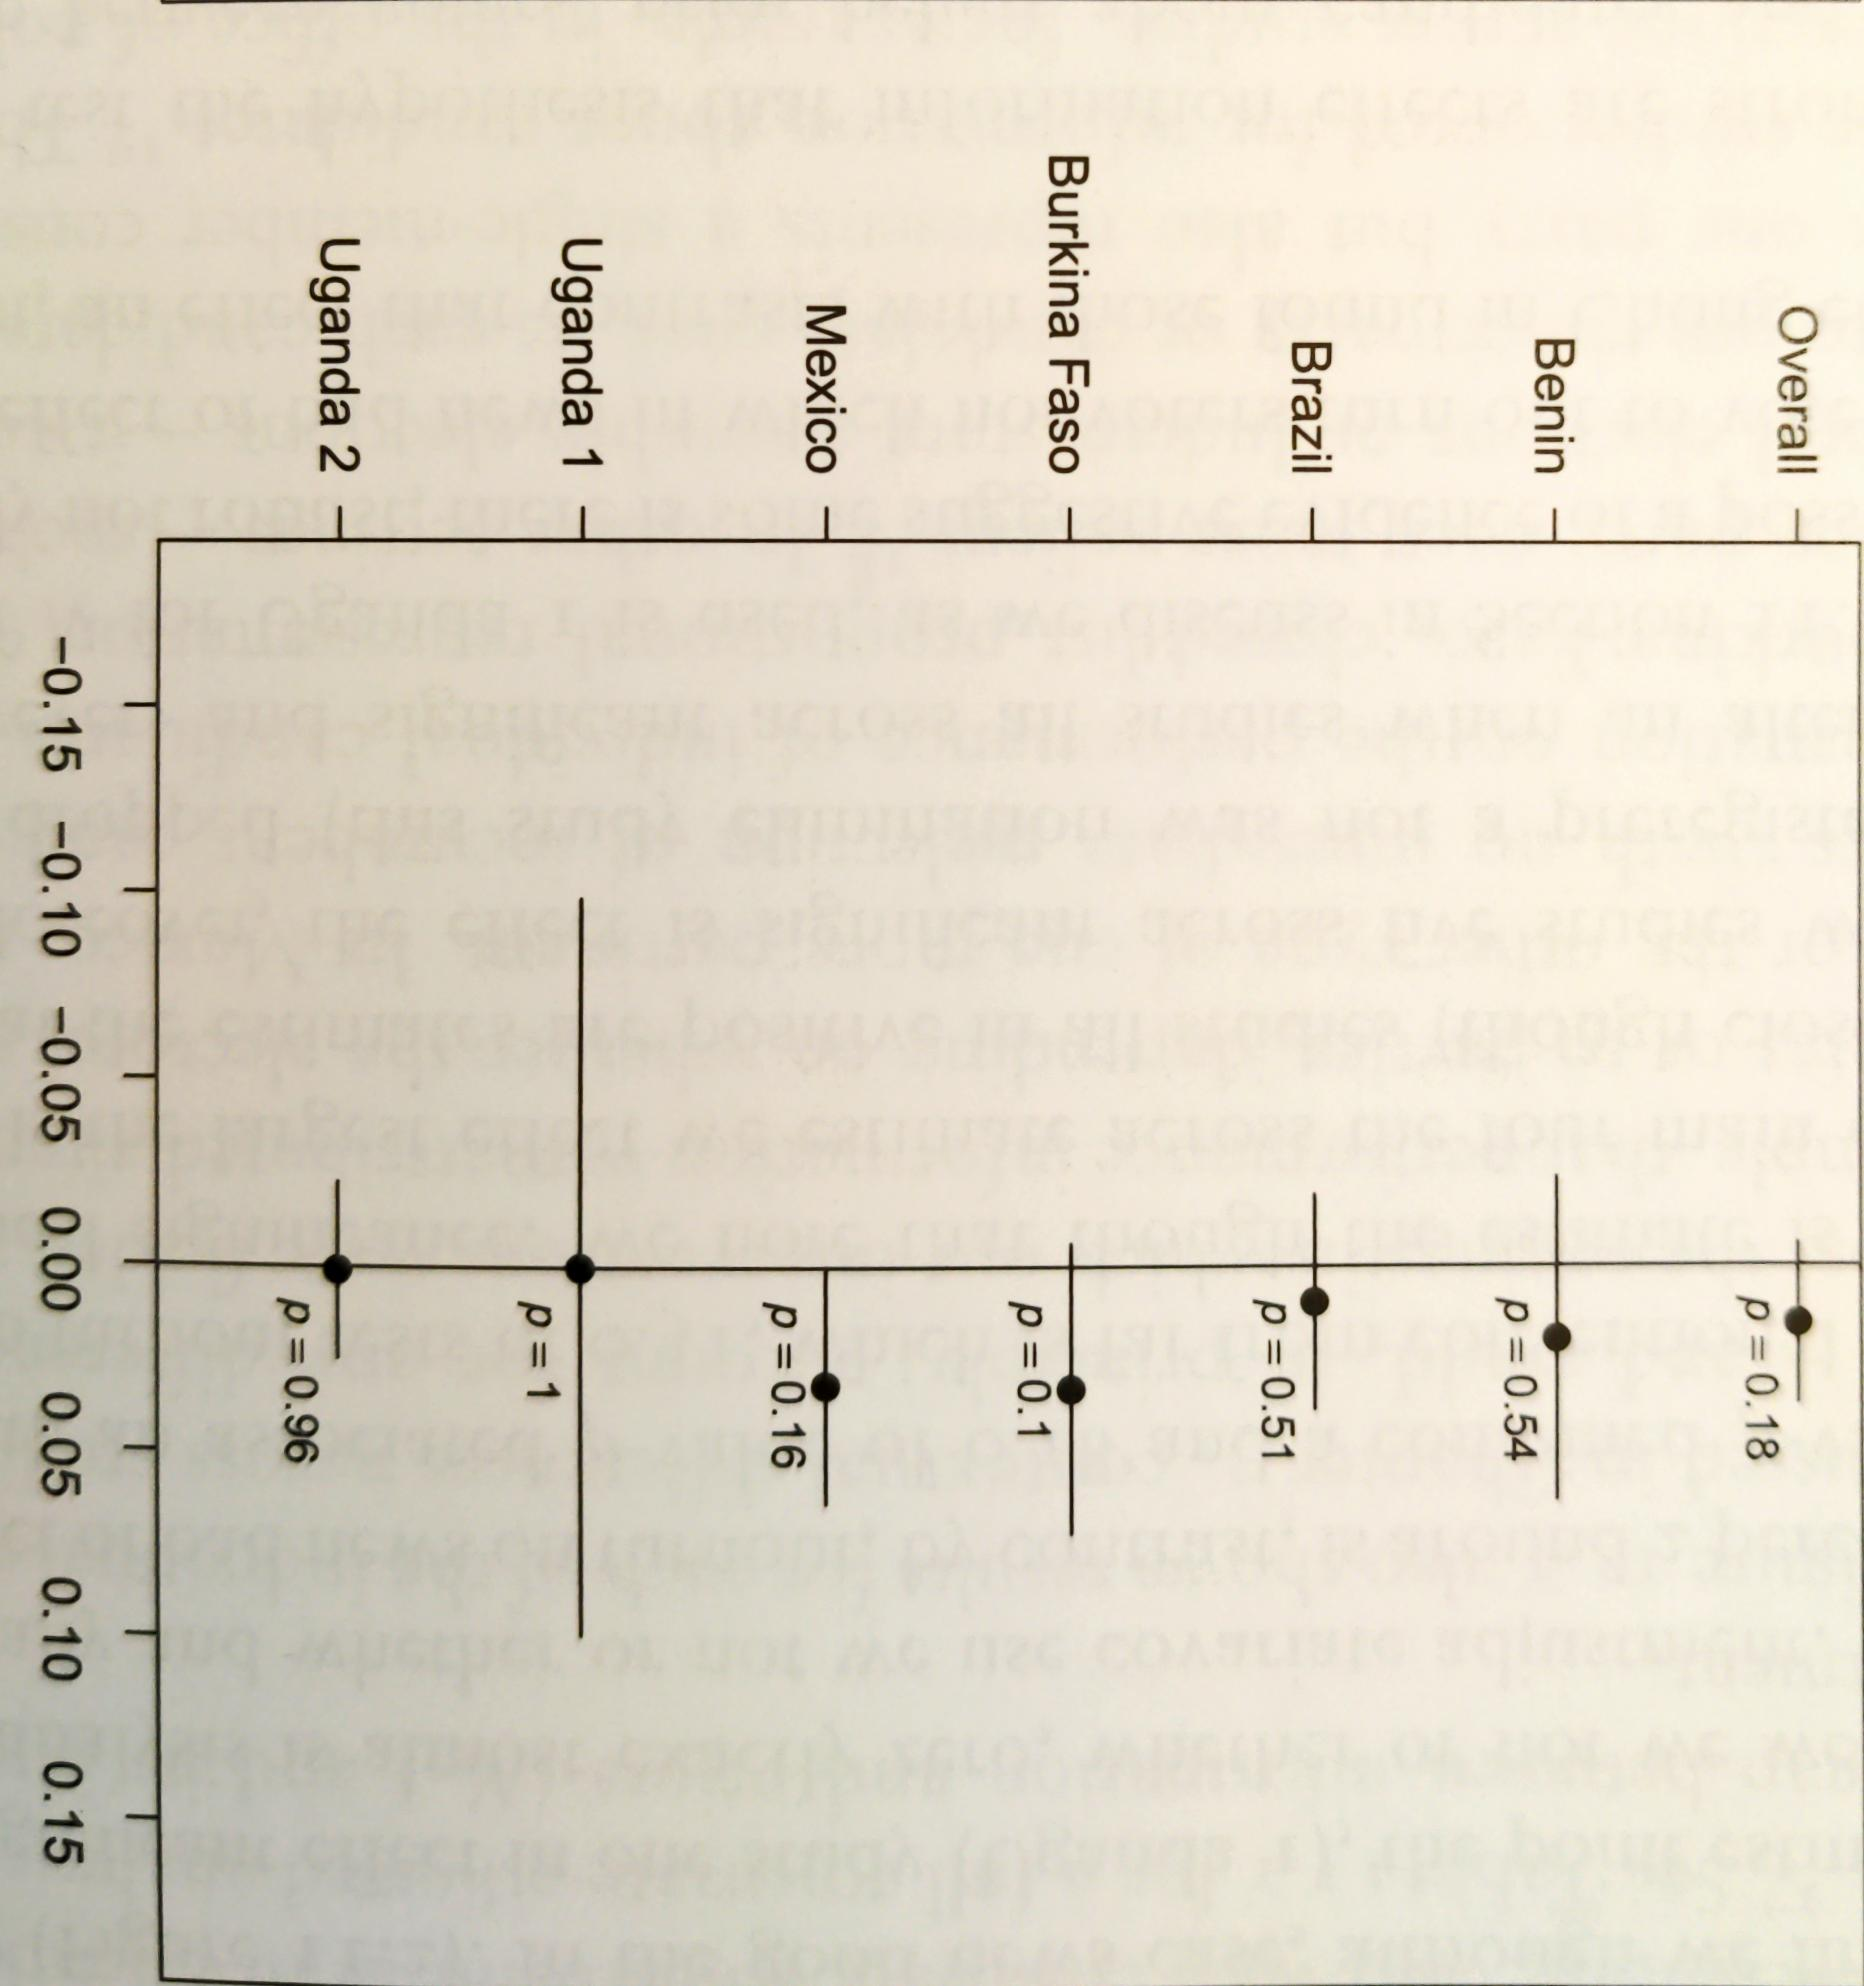
\includegraphics[scale=0.071,angle=90]{../04-figures/12/04-Good-news-turnout.jpg}
			\caption{Good news}
		\end{subfigure}
		\begin{subfigure}{0.47\linewidth}
			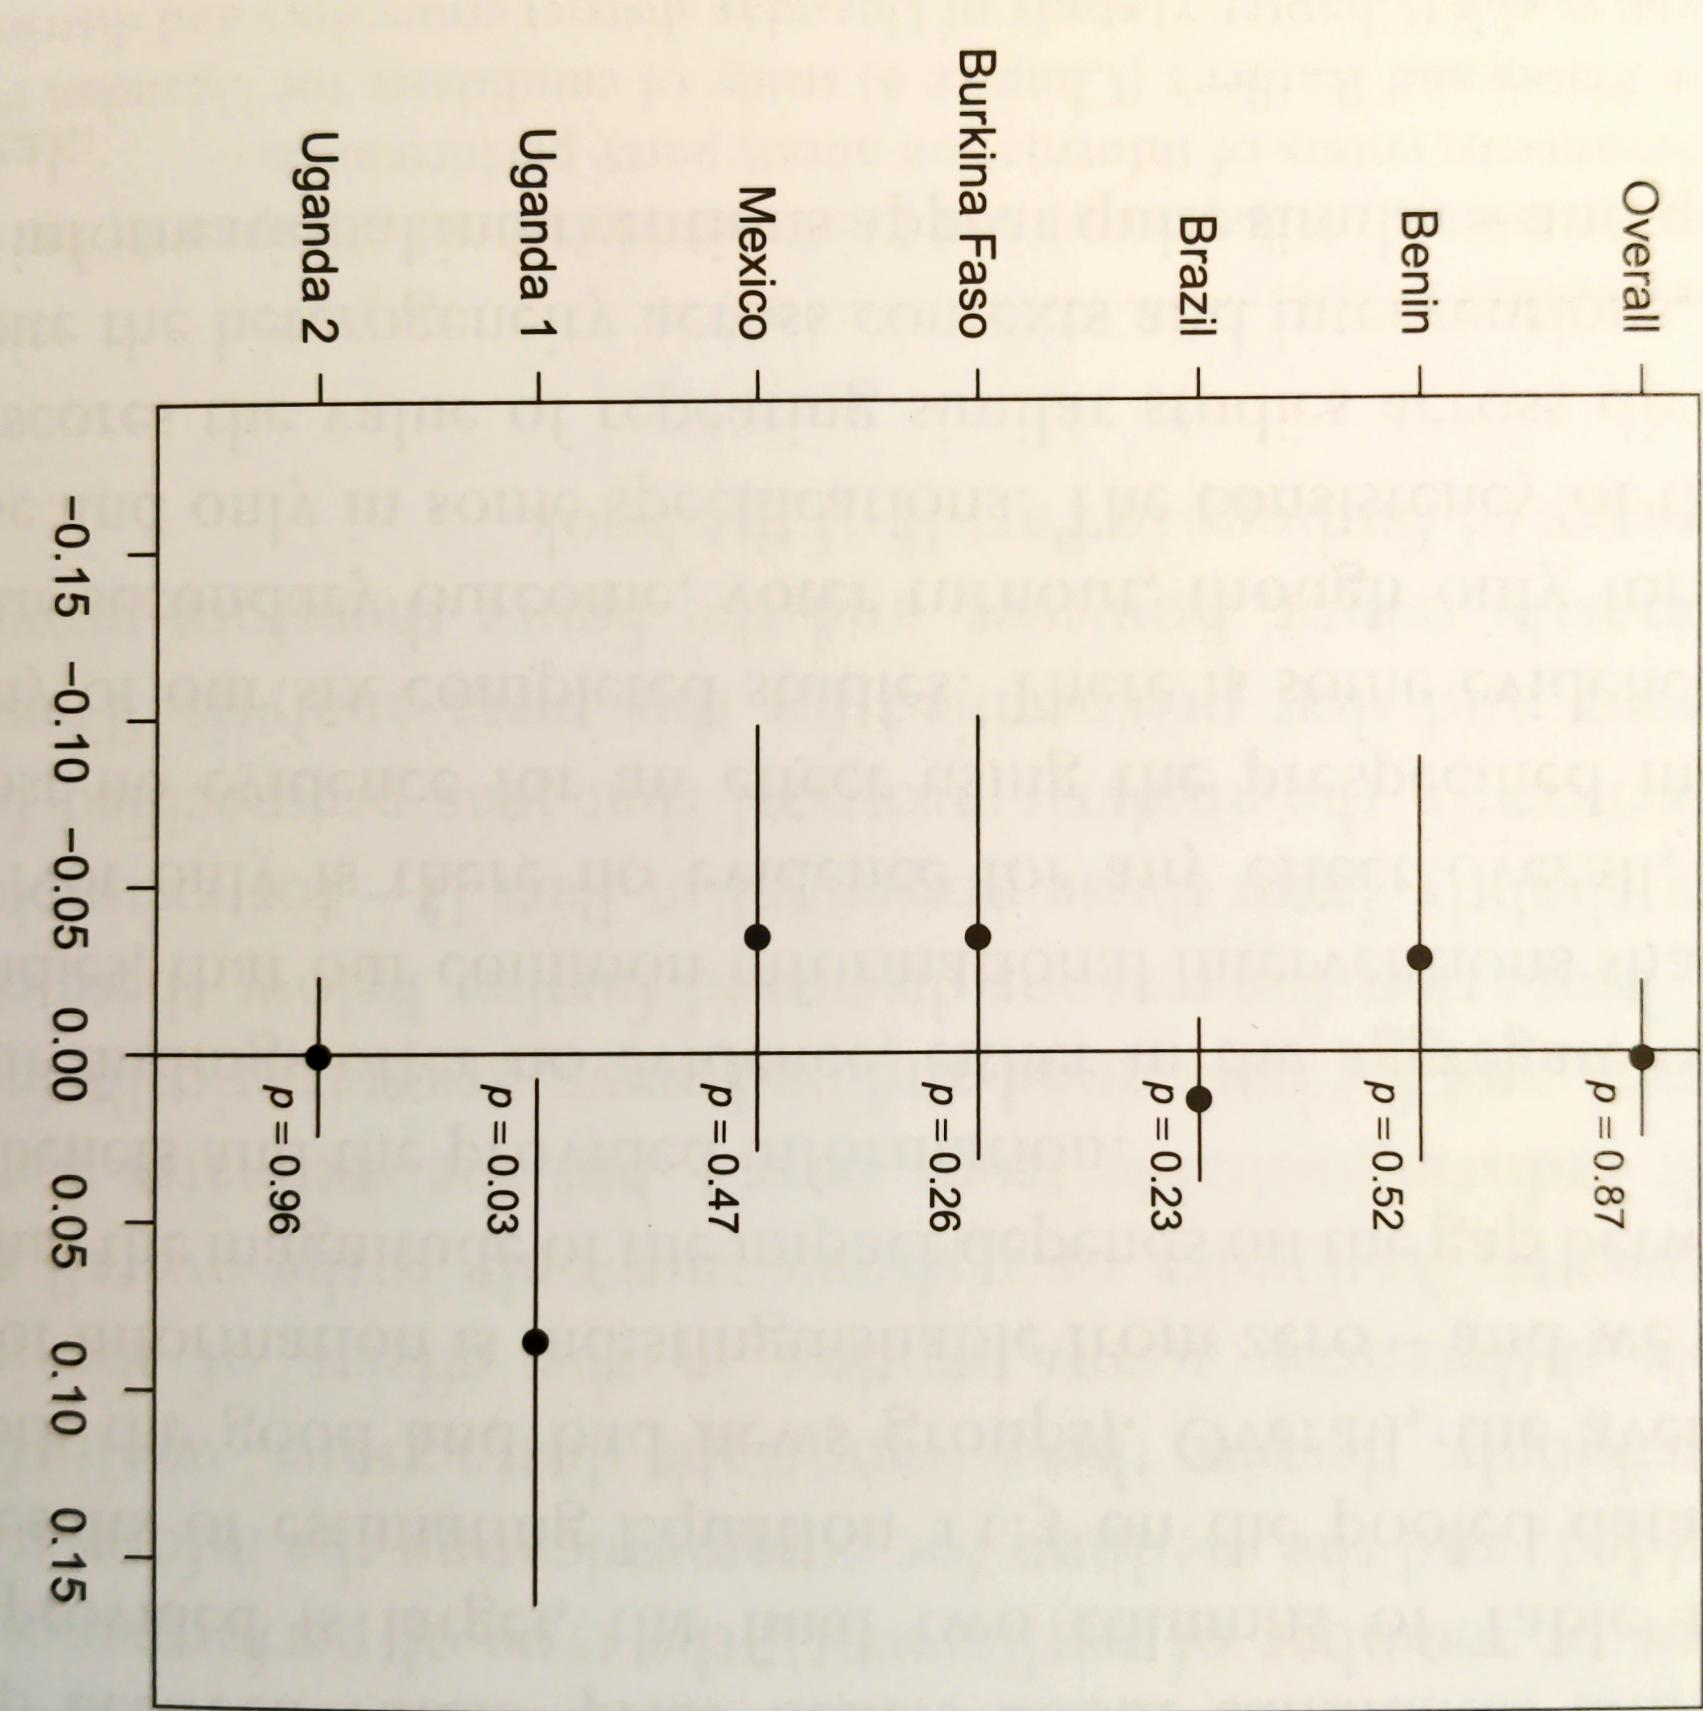
\includegraphics[scale=0.078,angle=90]{../04-figures/12/05-Bad-news-turnout.jpg}
			\caption{Bad news}
		\end{subfigure}
		\caption{Taken from \citeA{dunning_meta-analysis_2019}}
	\end{figure}
	
\end{frame}

\begin{frame}
	\frametitle{More Metaketa rounds}
	Currently-ongoing projects on:
	
	\begin{itemize}
		\item taxation (drivers of formalization, esp. information)
		\item natural resource governance (effects of strengthening community monitoring capacity)
		\item community policing (effectiveness in weak-state contexts)
		\item women involvement in consultative processes (mobilization factors)
	\end{itemize}
	\pause
	
	These, and similar other projects, take some steps toward greater generalizability of findings from RCTs.
	
\end{frame}


\subsection{External validity II}

\begin{frame}
	\frametitle{Self-selection everywhere}
	In an RCT researchers have high degree of control over treatment assignment.\bigskip
	
	A great benefit, but represents a vulnerability as well: treatment is assigned to people who in real life wouldn't take it.\bigskip
	\pause
	
	\textcolor{orange}{Examples}: media exposure effects on candidates for President, effects on tolerance from contact with out-group individuals.\bigskip
	\pause
	
	This isn't how people consume media or interact with others in real life---self-selection.
	
\end{frame}


\begin{frame}
	\frametitle{Patient preference trials}
	The ATE estimated from a RCT might only approximate poorly the effect in the population.\bigskip
	\pause
	
	\textcolor{orange}{Solution}: incorporate stated and revealed preferences over treatment arms in design \cite{knox_design_2019}.
	
	\begin{figure}
		\centering
		\visible<2>{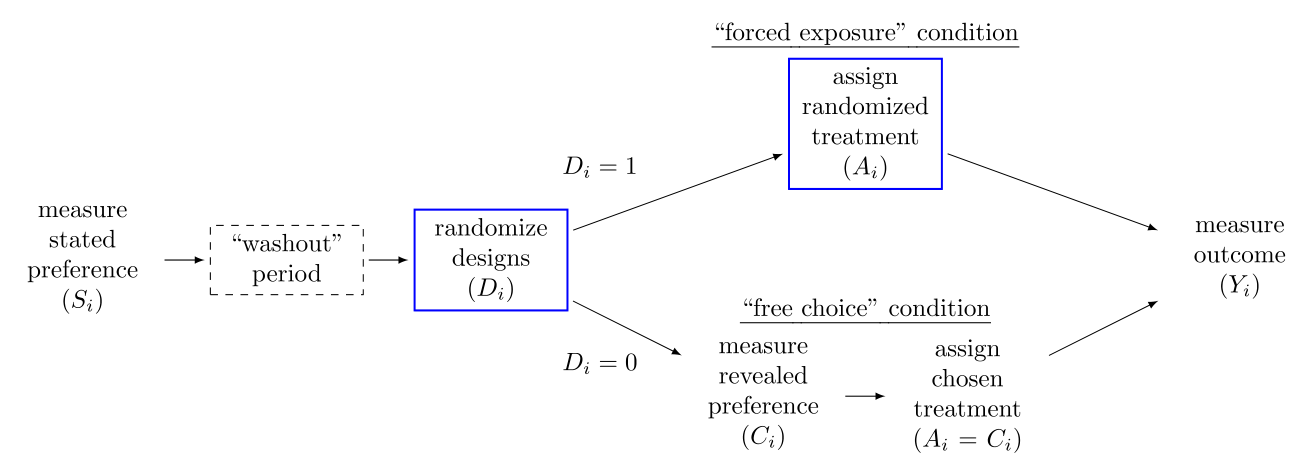
\includegraphics[scale=0.38]{../04-figures/12/08-Patient-preference.PNG}}
	\end{figure}
		
\end{frame}


\begin{frame}
	\frametitle{Patient preference trials}
	Design allows estimating multiple quantities:
	
	\begin{itemize}
		\item ATE: the standard treatment effect\pause
		\item ACTE: average choice-specific treatment effect---effect of treatment $t$ for those who would opt for something else in real life
	\end{itemize}\bigskip
	\pause
	
	Can provide information on what effects we might notice if we scale up an intervention.
	
\end{frame}


\begin{frame}
	\frametitle{Selective trials}
	Design related to that of \textit{selective trials} \cite{chassang_selective_2012}.\bigskip
	
	Hard to say why a treatment's measured effect is, for example, low:
	
	\begin{itemize}
		\item its true effect really is low\pause
		\item people \textit{believe} it's low $\Rightarrow$ don't use it
	\end{itemize}\bigskip
	\pause
	
	We cannot observe \textit{effort} with standard designs.
	
\end{frame}


\begin{frame}
	\frametitle{Selective trials}
	In these designs, participants can self-select into their preferred treatment arm at a cost (with probability dependent on willingness to pay).\bigskip
	\pause
	
	Provides information on treatment effects at different levels of belief in the treatment's benefits.
	
\end{frame}

\subsection{Aggregation challenges}

\begin{frame}
	\frametitle{From RCT estimates to macro dynamics}
	
	\begin{figure}
		\centering
		\caption{Relative power theory (updated)}
	\scalebox{0.7}{\begin{tikzcd}[node distance=1cm]
			\node (A) at (2,0) {\begin{tabular}{c} Relative \\ power \\ \end{tabular}}; 
			\node (B) at (2,-4) {\begin{tabular}{c} Self- \\ \ efficacy \\
			\end{tabular}};
			\node (D) at (8,-2) {\begin{tabular}{c} Participation \\ \end{tabular}};
			\node (C) at (-3,0) {\begin{tabular}{c} Economic \\ inequality \\ \end{tabular}};
			\draw [->, >=stealth, thick] (A)--(D);
			\draw [->, >=stealth, thick] (C)--(A);
			\draw [->, >=stealth, thick] (B)--(D);
			\draw [->, >=stealth, thick, shorten <=0.7cm] (A)--(B);
		\end{tikzcd}}
	\end{figure}\pause

	RCT result: accurate information about inequality in district $\Rightarrow$ lowered belief that voting can change anything.\pause
	
	What can we say about the macro-level phenomenon?
	
\end{frame}


\begin{frame}
	\frametitle{Alternative mediating pathways}
	If information is sole channel, we could get a sense of dynamics at macro level.\bigskip
	\pause
	
	If alternative pathways operate, e.g. parties changing mobilization strategies, we run into major difficulties \cite{humphreys_aggregation_2020}.\bigskip
	\pause
	
	General equilibrium effects come into play: if everyone's crop increases, prices might \textit{decrease}.\bigskip
	
\end{frame}


\begin{frame}
	\frametitle{Structural models}
	Moving from ``effects of causes'' to ``causes of effects'' \cite{holland_statistics_1986}.
	\pause
	
	\begin{equation}
		\tau_i = Y_i(1, M_i(1)) - Y_i(0, M_i(0))
	\end{equation}\pause

	Trying to better grasp the network of causal dynamics that generate $Y$, and how causal pathways in the network combine to produce effects in reality.\bigskip
	
	Valuable initial work by \citeA{pearl_external_2014}.
	
\end{frame}

\begin{frame}
	\begin{center}
		\Huge It was a pleasure having \textcolor{orange}{you} in the course!
	\end{center}
\end{frame}


% REFERENCES %

\begin{frame}[allowframebreaks, plain]
\frametitle{References}
\bibliographystyle{apacite}
\scriptsize\bibliography{../Bibliography}
\end{frame}

\end{document}
